%%%%%%%%%%%%%%%%%%%%%%%%%%%%%%%%%%%%%%%%%%%%%%%%%%%%%%%%%%%%%%%%%%%%%%%%%%%%%%%%
% ICML 2026 Position Paper
% Position: Web Agent Research Needs Capture-Replay Infrastructure
%%%%%%%%%%%%%%%%%%%%%%%%%%%%%%%%%%%%%%%%%%%%%%%%%%%%%%%%%%%%%%%%%%%%%%%%%%%%%%%%

\documentclass[letterpaper]{article}

% Required ICML style - use 'accepted' for camera-ready, remove for submission
\usepackage{icml2026}

% Recommended packages
\usepackage{microtype}
\usepackage{graphicx}
\usepackage{subcaption}
\usepackage{booktabs}
\usepackage{hyperref}
\usepackage{xcolor}
\usepackage{amsmath}
\usepackage{amssymb}

% For code listings
\usepackage{listings}
\lstset{
  basicstyle=\ttfamily\small,
  breaklines=true,
  frame=single,
  xleftmargin=0pt,
}

% URL handling (theHalgorithm is defined in icml2026.sty)

% Hyperref setup
\hypersetup{
  colorlinks=true,
  linkcolor=blue,
  citecolor=blue,
  urlcolor=blue
}

% Graphics path (figures are in parent directory)
\graphicspath{{../figures/}{figures/}}

% Short running title (must be in preamble, before \begin{document})
\icmltitlerunning{Position: Web Agent Research Needs Capture-Replay Infrastructure}

%%%%%%%%%%%%%%%%%%%%%%%%%%%%%%%%%%%%%%%%%%%%%%%%%%%%%%%%%%%%%%%%%%%%%%%%%%%%%%%%
% DOCUMENT START
%%%%%%%%%%%%%%%%%%%%%%%%%%%%%%%%%%%%%%%%%%%%%%%%%%%%%%%%%%%%%%%%%%%%%%%%%%%%%%%%

\begin{document}

\twocolumn[
\icmltitle{Position: Web Agent Research Needs Capture-Replay Infrastructure,\\Not More Handcrafted Replicas}

% For submission (anonymous)
\icmlsetsymbol{equal}{*}

\begin{icmlauthorlist}
\icmlauthor{Anonymous}{anon}
\end{icmlauthorlist}

\icmlaffiliation{anon}{Anonymous Institution}

\icmlcorrespondingauthor{Anonymous}{anonymous@email.com}

\icmlkeywords{Web Agents, Benchmarks, Capture-Replay, Browser Environments, Position Paper}

\vskip 0.3in
]

% This must go after \twocolumn for proper formatting
\printAffiliationsAndNotice{}

%%%%%%%%%%%%%%%%%%%%%%%%%%%%%%%%%%%%%%%%%%%%%%%%%%%%%%%%%%%%%%%%%%%%%%%%%%%%%%%%
% ABSTRACT
%%%%%%%%%%%%%%%%%%%%%%%%%%%%%%%%%%%%%%%%%%%%%%%%%%%%%%%%%%%%%%%%%%%%%%%%%%%%%%%%

\begin{abstract}
\textbf{This is a position paper.} We argue that web agent research should replace handcrafted website replicas with capture-replay infrastructure that turns real expert demonstrations into reusable, offline environments. Current benchmarks require heavy engineering yet cover a narrow, economically unrepresentative slice of web work, while proprietary environment providers concentrate access. Capture-replay offers a scalable alternative: a single expert session can produce a complete environment in minutes, grounded in real workflows and shareable via open-source tooling. We analyze the benchmark landscape and its cost structure, and present TRACE, a proof-of-concept pipeline that works on production sites including authenticated flows. We discuss limitations (reduced exploration, legal and ethical constraints, and replay determinism) and argue they are tractable through additional collection and community norms. We conclude with a call to action to redirect investment away from handcrafted replicas and toward capture-replay, and to document environment construction costs to enable fair methodological comparisons.
\end{abstract}

%%%%%%%%%%%%%%%%%%%%%%%%%%%%%%%%%%%%%%%%%%%%%%%%%%%%%%%%%%%%%%%%%%%%%%%%%%%%%%%%
% SECTION 1: INTRODUCTION
%%%%%%%%%%%%%%%%%%%%%%%%%%%%%%%%%%%%%%%%%%%%%%%%%%%%%%%%%%%%%%%%%%%%%%%%%%%%%%%%

\section{Introduction}
\label{sec:introduction}

\begin{quote}
\emph{``Web agents are hill climbing in the wrong direction.''}
\end{quote}

The past two years have witnessed remarkable progress in language-model agents for web and computer use. Systems built on frontier models can now navigate complex websites, fill forms, execute multi-step workflows, and retrieve information across diverse domains \citep{song2025bearcubs, wei2025browsecomp, murty2024nnetscape, maia2023gaia, zhang2023mind2web, li2025mind2web2, zhou2023webarena, garg2025real, xie2024osworld, xu2024theagentcompany, he2024webvoyager, drouin2024workarena}. Benchmarks such as Mind2Web, WebArena, WebVoyager, WorkArena, REAL, OSWorld, BEARCUBS, BrowseComp, and TheAgentCompany have provided standardized evaluation environments that enable reproducible comparisons and have driven rapid capability improvements.

Yet beneath this progress lies a troubling structural problem: \textbf{the environments we use to train and evaluate web agents bear little resemblance to the tasks that would make these agents economically valuable.} The majority of benchmark tasks fall into categories we characterize as ``deep research'' (trivia-style multi-hop questions that rarely require browser automation), ``information seeking'' (simple lookups that could often be answered by a search engine), or ``atomic execution'' (short, isolated actions like clicking a button or filling a single field). Long-horizon, multi-step workflows that mirror real paid work (booking complex travel itineraries, configuring enterprise SaaS tools, executing financial transactions, managing e-commerce operations) remain dramatically underrepresented. More importantly, most benchmarks are not collected from people doing paid work; they are task templates designed for evaluability rather than traces of real economic activity.

This is not an oversight. It reflects a fundamental constraint: \textbf{handcrafted environments are extraordinarily expensive to build.}

\paragraph{Our position:} The web agent research community should replace handcrafted replicas with capture-replay infrastructure. Rather than building website replicas, we should record experts completing tasks on live websites and transform those recordings into reusable, offline environments. A single expert demonstration can produce a complete environment in minutes, compared to the hours or days required to handcraft a replica. The tools exist; the decision is whether we continue paying the replica tax or move the field forward.

Consider the costs documented in recent benchmark papers:

\begin{table}[h]
\caption{Environment construction costs for prominent benchmarks.}
\label{tab:costs}
\vskip 0.1in
\centering
\small
\begin{tabular}{@{}lrl@{}}
\toprule
\textbf{Benchmark} & \textbf{Tasks} & \textbf{Reported Effort} \\
\midrule
WebArena & $\sim$812 & Months of development; self-hosting \\
 & & four functional website replicas \\
OSWorld & $\sim$369 & Hand-annotated tasks with initial \\
 & & state scripting and custom evaluators \\
TheAgentCompany & $\sim$175 & \textbf{3,000 person-hours} by 21 \\
 & & contributors over two months \\
REAL & $\sim$112 & Deterministic replicas of 11 real \\
 & & websites with custom harnesses \\
\bottomrule
\end{tabular}
\end{table}

TheAgentCompany's transparent reporting is particularly illuminating: building 175 realistic ``employee-style'' tasks required 3,000 person-hours---the equivalent of 1.5 full-time engineers working for an entire year. The project involved 21 contributors including software engineers and project managers, with complex tasks requiring more than 10 hours each to design, implement, test, and verify. And these are among the most resource-rich academic teams in the field.

\textbf{The implication is stark:} at current construction costs, the academic community cannot build environments at the scale needed to cover the long tail of economically valuable browser tasks. We can produce hundreds of tasks, perhaps low thousands with extraordinary effort, but the space of valuable web workflows spans millions of distinct patterns across hundreds of thousands of websites.

These costs are not only financial. They consume scarce research time that could otherwise go toward agent design, failure analysis, and iteration. And because realistic environment construction is so expensive, evaluation suites remain small and often collapse to binary success metrics, which limits error analysis and makes it difficult to diagnose where, why, and how models fail.

This gap has not gone unnoticed by industry. A growing ecosystem of startups now builds browser environments for AI agent training \citep{mechanize, plato, agiinc, kaizen}. The business models vary: some host live environments, others deliver static datasets, and some offer both. What they share is a focus on creating replica websites and simulated workflows where AI agents can learn through reinforcement learning without triggering blocking mechanisms on real sites.

The scale of investment is remarkable. According to \emph{The Information}, Anthropic has discussed spending more than \$1 billion on RL environments over the next year \citep{zeff2025silicon}. Data-labeling giants like Scale AI, Surge, and Mercor are pivoting resources toward environment construction, with Surge reportedly generating \$1.2 billion in revenue last year from AI lab contracts and recently spinning up a dedicated internal organization for RL environments. Mechanize, a startup focused exclusively on environments, offers software engineers \$500,000 salaries to build them, far exceeding typical data-labeling contractor rates. Andreessen Horowitz general partner Jennifer Li summarized the landscape: ``All the big AI labs are building RL environments in-house... but AI labs are also looking at third-party vendors that can create high-quality environments.''

Leading AI labs treat these environments as core training infrastructure. \textbf{Browser environments have become a strategic asset: valuable, proprietary, and concentrated in the hands of well-funded organizations.}

\textbf{The field is at an inflection point.} Three trends are converging: (1) agents are becoming capable enough that evaluation on short, synthetic tasks no longer discriminates between systems, creating demand for long-horizon, realistic environments; (2) the cost of building such environments has created a two-tier ecosystem where frontier labs invest billions while academic groups work with hundreds of tasks; and (3) the resulting concentration raises safety concerns, as independent researchers cannot study systems trained on environments they cannot access. If the community does not change course, the gap will widen and become structural.

We believe this trajectory is problematic for the field. When the ability to train and iterate on realistic web agents depends on access to expensive proprietary infrastructure, the research community's capacity for independent investigation is constrained. Open science suffers. Reproducibility suffers. And the concentration of capability in a small number of actors raises broader concerns about the development trajectory of increasingly powerful autonomous systems. This issue affects not only academic groups, but also open-source LM companies operating on budgets that are tiny relative to frontier labs.

\textbf{This paper argues for an alternative approach: capture-replay.}

The core idea is simple: rather than handcrafting website replicas, we record an expert completing a task on a live website and transform that recording into a self-contained environment that can be replayed offline. A single expert demonstration (taking minutes to perform) produces a complete environment bundle including DOM states, network responses, screenshots, and interaction logs. Agents can then be evaluated (and potentially trained) against this frozen snapshot without contacting the live web.

Capture-replay is not a new concept in software engineering. Record-and-replay debugging, network mocking, and browser automation testing have used similar techniques for decades. But its application to web agent research has been surprisingly limited. We argue this represents a significant missed opportunity.

To demonstrate feasibility, we developed TRACE (Trajectory Recording and Capture Environments), an open-source capture-replay pipeline. Building robust tooling required approximately 300 hours of engineering effort: analyzing hundreds of captured sessions, developing URL canonicalization heuristics, and iterating on replay matching. But once built, the tooling amortizes: we captured six diverse environments (GitHub, Amazon, Airbnb, Kayak, Uniqlo, Ultimate Guitar) in approximately 40 minutes of total collection time, including retries and quality checks. This is roughly 6--7 minutes per task versus the 10+ hours per task reported for handcrafted benchmarks like TheAgentCompany.

We emphasize ``replace'' deliberately. Handcrafted replicas consume scarce human capital but are not required to achieve determinism, controlled variation, or breadth. Those properties can be achieved by capture-replay at scale: multi-trajectory collection, record-on-miss expansion, and post-processing that enables controlled perturbations. The community's near-exclusive focus on replicas has slowed progress and narrowed evaluation; we argue the field should move past them.

The remainder of this paper develops this argument in detail:

\begin{itemize}
    \item \textbf{Section~\ref{sec:landscape}} presents a taxonomy of existing benchmarks, revealing systematic gaps in economically valuable task coverage and analyzing the cost structure of current approaches.
    \item \textbf{Section~\ref{sec:case}} articulates the case for capture-replay, describing its potential advantages and presenting TRACE as a proof-of-concept implementation.
    \item \textbf{Section~\ref{sec:counterarguments}} addresses alternative views and counterarguments, including concerns about exploration latitude, legal and ethical considerations, and technical feasibility.
    \item \textbf{Section~\ref{sec:call}} presents a concrete call to action with specific recommendations for researchers, benchmark creators, and the broader community.
\end{itemize}

%%%%%%%%%%%%%%%%%%%%%%%%%%%%%%%%%%%%%%%%%%%%%%%%%%%%%%%%%%%%%%%%%%%%%%%%%%%%%%%%
% SECTION 2: CURRENT LANDSCAPE
%%%%%%%%%%%%%%%%%%%%%%%%%%%%%%%%%%%%%%%%%%%%%%%%%%%%%%%%%%%%%%%%%%%%%%%%%%%%%%%%

\section{The Current Landscape: Expensive Replicas, Limited Coverage}
\label{sec:landscape}

\subsection{A Taxonomy of Browser Agent Benchmarks}

To understand the current state of web agent environments, we systematically analyzed eleven prominent benchmarks across three dimensions: \textbf{task category} (what kind of work the agent performs), \textbf{task horizon} (how many steps or how much time tasks typically require), and \textbf{economic grounding} (whether tasks resemble work someone would pay to have completed).

\begin{table*}[t]
\caption{Taxonomy of existing web agent benchmarks. We observe a clear pattern: benchmarks with high economic grounding (TheAgentCompany, WorkArena, parts of REAL) require the most construction effort, while scalable benchmarks (Mind2Web, BrowseComp) tend toward tasks with limited economic value.}
\label{tab:taxonomy}
\vskip 0.1in
\centering
\small
\begin{tabular}{@{}llllp{5.5cm}@{}}
\toprule
\textbf{Benchmark} & \textbf{Category} & \textbf{Horizon} & \textbf{Econ. Grounding} & \textbf{Key Limitation} \\
\midrule
GAIA & Deep research & Medium & Low & General-assistant QA; many tasks not web-specific \\
BEARCUBS & Info seeking & Short--Medium & Low & QA-only; no state-changing actions; small (111 tasks) \\
BrowseComp & Deep research & Long & Low & QA-only; short answers; open-web drift \\
Mind2Web 2 & Deep research & Long & Low & Agentic search QA; LLM-as-judge evaluation \\
Mind2Web & Info seeking / Exec & Short--Medium & Medium & Live-web trajectories; action-matching eval; no deterministic env \\
WebVoyager & Info seeking / Exec & Medium & Low--Medium & Live websites; GPT-4V-based eval; limited domain coverage \\
WebArena & Execution & Medium & Medium & Replica sites; limited domains; high construction cost \\
REAL & Execution & Short--Medium & Medium--High & Deterministic replicas; limited task count and domains \\
OSWorld & Execution & Short--Medium & Medium & Desktop-focused; heavy state setup and evaluators \\
WorkArena & Execution & Short--Medium & High & Single platform (ServiceNow); small (33 tasks); remote-hosted \\
TheAgentCompany & Execution & Medium & High & Realistic workflows but extraordinarily expensive to build \\
\bottomrule
\end{tabular}
\end{table*}

Several patterns emerge from this analysis:

\paragraph{Pattern 1: The effort-value tradeoff.} Benchmarks that emphasize economically realistic tasks (TheAgentCompany, WorkArena, REAL) require dramatically more construction effort than those emphasizing information retrieval or synthetic reasoning (BrowseComp, GAIA). This is not coincidental. Realistic execution tasks require functional environments with state that actually changes, authentication flows that work, and evaluation criteria that verify real outcomes.

\paragraph{Pattern 2: Horizon compression.} Even benchmarks labeled as ``long-horizon'' often consist of relatively short interaction sequences when measured in actual steps. Mind2Web 2 explicitly analyzed this phenomenon, finding that most existing benchmarks concentrate on short-horizon tasks \citep{li2025mind2web2}. Long-horizon, multi-session workflows that characterize real knowledge work remain rare.

\paragraph{Pattern 3: Horizon costs explode.} As agents improve, the field is pushing toward longer-horizon evaluations (e.g., METR's work on measuring ability to complete long tasks \citep{metr2025}). But handcrafting long-horizon tasks scales poorly: if some tasks already require 10+ hours to design and verify, the idea of 12-hour, multi-day, or week-long workflows is untenable. Replica construction cannot keep pace with the horizon lengths we need to measure.

\paragraph{Pattern 4: Domain concentration.} Existing benchmarks heavily favor a small set of domains: e-commerce, content management, developer tools, and travel booking appear repeatedly, while vast categories of economically important web work (financial services, healthcare portals, government services, enterprise SaaS, professional services) remain largely uncovered.

\paragraph{Pattern 5: The live-web evaluation problem.} Benchmarks that evaluate on live websites (Mind2Web, BrowseComp, BEARCUBS, WebVoyager) face continuous validity challenges as the web changes. Those that avoid this through replicas (WebArena, REAL) gain reproducibility but lose coverage and realism.

\subsection{The Cost Structure of Environment Construction}

Why are realistic browser environments so expensive to build? The costs compound across multiple dimensions:

\paragraph{Website replication costs.} Creating a functional replica of even a moderately complex website requires reverse-engineering its interaction model, implementing sufficient backend logic to respond meaningfully to agent actions, and maintaining consistency as the original site evolves. REAL's approach (deterministic simulations of 11 real websites) required building custom evaluation harnesses that mix programmatic checks with LLM-based judgment \citep{garg2025real}.

\paragraph{State initialization costs.} Realistic tasks often require specific preconditions: items in a shopping cart, emails in an inbox, projects configured in a particular way. OSWorld's task suite required extensive scripting to establish correct initial states for each of its 370 tasks \citep{xie2024osworld}. TheAgentCompany built an entire simulated company environment with interconnected services \citep{xu2024theagentcompany}.

\paragraph{Evaluation complexity costs.} When tasks have multiple valid solutions or require judgment about partial completion, evaluation itself becomes a substantial engineering challenge. The field has increasingly turned to LLM-as-a-judge approaches, but these introduce their own costs, biases, and reproducibility concerns \citep{xue2025illusion}.

\paragraph{Maintenance costs.} The web changes constantly. Benchmarks evaluated on live sites require ongoing curation to verify task validity. Replica-based benchmarks must track upstream changes if they aim to remain representative.

\paragraph{Credential and access costs.} Many economically valuable tasks require authenticated access to real services. Benchmarks either avoid these tasks, use synthetic accounts with limited functionality, or require evaluators to provide their own credentials. Each approach constrains coverage or reproducibility.

\subsection{The Concentration of Environment Access}

The expense of environment construction has predictable consequences for who can build and access high-quality environments.

As discussed above, a commercial ecosystem has emerged to fill this gap. These providers offer browser environments through various models: some host live replicas, others deliver packaged datasets, and some provide both. The environments enable something impossible on real websites: running thousands of AI agents simultaneously through trial-and-error learning without being blocked.

Leading AI labs use these commercial environments for training and evaluating their web agents. As frontier labs have exhausted most available text data for pretraining, reinforcement learning in simulated environments has become increasingly important. With per-task costs in the thousands to tens of thousands of dollars, these environments represent substantial investments, but ones that well-capitalized organizations can afford while academic groups generally cannot.

\textbf{The result is a two-tier system:} well-funded labs train agents on high-quality, realistic environments that they cannot share, while the academic community and open-source LM companies work primarily with the limited set of open benchmarks. This concentration raises concerns about:

\begin{enumerate}
    \item \textbf{Reproducibility:} If state-of-the-art results depend on proprietary training environments, the research community cannot fully verify or build upon them.
    \item \textbf{Diversity:} Concentrated environment access may lead to agents that excel on specific task distributions while failing on the broader diversity of real-world needs.
    \item \textbf{Safety:} Independent safety research requires access to the same environments used for capability development; concentration of access constrains this.
\end{enumerate}

%%%%%%%%%%%%%%%%%%%%%%%%%%%%%%%%%%%%%%%%%%%%%%%%%%%%%%%%%%%%%%%%%%%%%%%%%%%%%%%%
% SECTION 3: THE CASE FOR CAPTURE-REPLAY
%%%%%%%%%%%%%%%%%%%%%%%%%%%%%%%%%%%%%%%%%%%%%%%%%%%%%%%%%%%%%%%%%%%%%%%%%%%%%%%%

\section{The Case for Capture-Replay}
\label{sec:case}

\subsection{Core Concept}

Capture-replay inverts the environment construction process. Rather than building a website replica and then defining tasks on it, we:

\begin{enumerate}
    \item \textbf{Capture:} An expert performs a real task on a live website while an instrumented browser records everything: DOM states, network traffic, user interactions, screenshots, and video.
    \item \textbf{Process:} A post-processing pipeline transforms raw captures into clean, reusable artifacts: high-level action sequences (a standardized tool-call DSL), extracted credentials (for secure handling), semantic checkpoints (for partial-credit evaluation), and filtered network logs (removing analytics and non-essential traffic).
    \item \textbf{Replay:} A replay engine serves the captured assets locally, allowing agents to interact with a frozen snapshot of the original session without contacting the live web.
\end{enumerate}

\subsection{Advantage 1: Scalability}

The most significant advantage of capture-replay is speed. \textbf{A single expert demonstration produces a complete environment in the time it takes to perform the task.}

Our proof-of-concept implementation (TRACE) captured six diverse tasks across GitHub, Amazon, Airbnb, Kayak, Uniqlo, and Ultimate Guitar in about 40 minutes of total collection time including retries (about 6:40 per task). Each capture produced hundreds of HTTP responses, dozens of DOM snapshots, and complete interaction logs---artifacts that would require days or weeks to handcraft.

This changes the economics of environment construction fundamentally. At capture-replay speeds:
\begin{itemize}
    \item A single researcher could produce hundreds of environments per week
    \item Crowdsourced collection becomes feasible (we built a desktop app for non-technical collectors)
    \item The long tail of websites becomes accessible: any site an expert can use can become an environment
\end{itemize}

\subsection{Advantage 2: Economic Grounding}

Capture-replay environments are grounded in real tasks by construction. When an expert books an actual flight, configures a real SaaS tool, or completes a genuine e-commerce transaction, the resulting environment captures a workflow that someone demonstrably values enough to perform.

This contrasts with the synthetic task design required for replica-based benchmarks, where researchers must imagine what tasks would be valuable and then construct environments to support them. Capture-replay enables a different paradigm: \textbf{find people doing economically valuable work, record them, and build environments from their actual workflows.}

\subsection{Advantage 3: Democratization}

Open-source capture-replay tooling can break the concentration of environment access. Any researcher with a browser can record environments from any website they can access. No proprietary infrastructure required, no licensing fees, no vendor lock-in.

This is not merely theoretical. TRACE is released as open-source software (URL redacted for double-blind review), and its captured environments are published on a public dataset host (URL redacted for double-blind review). The tooling is designed for extensibility: researchers can adapt it to their domains, contribute improvements, and build shared infrastructure without depending on commercial providers.

\subsection{TRACE: A Proof of Concept}

To demonstrate that capture-replay is technically feasible on modern production websites, we developed TRACE (Trajectory Recording and Capture Environments), an open-source pipeline implementing the full capture-process-replay workflow.

TRACE implements three core components: (1) a \textbf{collection} system using a stealth-configured Playwright browser that records DOM states, network traffic, user interactions, screenshots, and browser storage; (2) a \textbf{post-processing} pipeline that converts raw events to a standardized action DSL, extracts credentials for secure handling, identifies semantic checkpoints, and filters non-essential traffic; and (3) a \textbf{replay} engine that serves captured assets offline with deterministic request matching. Full implementation details are provided in Appendix~\ref{app:implementation}.

\paragraph{Demonstration dataset.} We release six captured environments spanning GitHub, Amazon, Ultimate Guitar (authenticated flows with login), and Uniqlo, Kayak, Airbnb (unauthenticated). These cover e-commerce, travel search, social coding, and media sites, including sensitive interactions like payment flows. Statistics are provided in Appendix~\ref{app:statistics}.

The dataset is intentionally small: six tasks demonstrates \emph{feasibility}, not comprehensive coverage. Building TRACE required approximately 300 hours of engineering effort, but once built, the six environments were captured in about 40 minutes total ($\sim$6--7 minutes per task). This asymmetry (high tooling cost, low marginal collection cost) is precisely why capture-replay scales where replicas do not.

%%%%%%%%%%%%%%%%%%%%%%%%%%%%%%%%%%%%%%%%%%%%%%%%%%%%%%%%%%%%%%%%%%%%%%%%%%%%%%%%
% SECTION 4: ALTERNATIVE VIEWS AND COUNTERARGUMENTS
%%%%%%%%%%%%%%%%%%%%%%%%%%%%%%%%%%%%%%%%%%%%%%%%%%%%%%%%%%%%%%%%%%%%%%%%%%%%%%%%

\section{Alternative Views and Counterarguments}
\label{sec:counterarguments}

A position paper must engage seriously with opposing views. We address the most significant counterarguments to capture-replay:

\subsection{``Capture-replay limits agent exploration''}

\paragraph{The concern:} Replica-based environments allow agents to explore freely: taking different paths, making mistakes, recovering from errors. Captured environments are constrained to the specific trajectory recorded; if an agent deviates, the replay may lack the network responses needed to continue.

\paragraph{Our response:} This is not a fundamental limitation. The low cost of collection makes coverage of alternative paths a data problem, not an environment-construction problem. Two practical mechanisms address exploration directly:

\begin{enumerate}
    \item \textbf{Multi-trajectory collection.} Capture multiple expert paths for the same task. These provide recovery behaviors and legitimate alternatives without any hand-built replica.
    \item \textbf{Deterministic branching for exploration.} Replay can expose captured branches deterministically, allowing beam-search-style exploration over alternative paths. When an agent hits a missing branch, record-on-miss collection adds it and expands the environment.
\end{enumerate}

In short, exploration constraints are solvable with more capture and deterministic branching, not a reason to keep handcrafted replicas.

\subsection{``Legal and ethical concerns around captured content''}

\paragraph{The concern:} Capturing and redistributing website content raises legal questions (copyright, terms of service) and ethical questions (privacy, consent, potential for misuse).

\paragraph{Our response:} These concerns are legitimate and require careful attention. We advocate for:

\begin{enumerate}
    \item \textbf{Credential extraction and substitution.} TRACE's pipeline separates credentials from captured content, allowing environments to be shared without exposing real passwords or tokens.
    \item \textbf{PII redaction.} Post-processing should identify and redact personally identifiable information beyond credentials.
    \item \textbf{Restricted distribution.} Not all captured environments should be publicly released. Research-use agreements, access controls, and clear licensing can balance openness with responsibility.
    \item \textbf{Ethical guidelines.} The community should develop shared norms around what captures are appropriate. We propose guidelines in Appendix~\ref{app:ethics}.
\end{enumerate}

\textbf{Importantly, replica-based benchmarks face analogous concerns that are often overlooked.} WebArena clones the visual design and interaction patterns of Reddit, GitLab, and shopping sites. REAL builds ``deterministic simulations'' that reproduce real website behavior. These replicas copy copyrighted UI designs, reverse-engineer proprietary interaction models, and redistribute structural representations of commercial products. Capture-replay does not introduce novel legal risk categories; it inherits the same ambiguities that replica builders have navigated for years.

\subsection{``Training requires more exploration than evaluation''}

\paragraph{The concern:} TRACE is currently validated for evaluation, not RL training. Training via reinforcement learning requires exploration, trial-and-error, and feedback from mistakes. Captured environments cannot provide negative rewards for failed actions or support recovery from off-trajectory states.

\paragraph{Our response:} We see no fundamental barrier to training use, only engineering and data scale challenges. Consider what multi-trajectory capture-replay provides:

\begin{enumerate}
    \item \textbf{A graph of valid transitions, not a single path.} With sufficient trajectory diversity, captured environments form a state-action graph suitable for offline RL and batch RL methods.
    \item \textbf{Graded reward signals via checkpoints.} TRACE's checkpoint system enables partial-credit feedback even when agents fail the final goal.
    \item \textbf{Imitation learning and behavioral cloning.} Captured expert demonstrations are directly usable for learning from demonstration.
    \item \textbf{Record-on-miss expansion.} When agents hit uncaptured branches, the missing transitions can be recorded and added.
\end{enumerate}

The key question is data scale: how many trajectories are needed for effective RL? This is empirical. We also note that \textbf{evaluation is the more urgent bottleneck}---most academic groups cannot evaluate on realistic long-horizon tasks because the environments do not exist.

\subsection{``The modern web actively resists being captured''}

\paragraph{The concern:} Websites deploy sophisticated anti-automation measures: CAPTCHA challenges, bot detection, device fingerprinting, behavioral analysis, and rate limiting.

\paragraph{Our response:} This is true, and one reason TRACE required substantial engineering effort. We found that:

\begin{enumerate}
    \item \textbf{Many high-value sites are capturable} with sufficient engineering. Stealth browser configuration and realistic interaction timing enabled successful capture across all six demonstration sites.
    \item \textbf{Anti-bot measures vary widely in sophistication.} The landscape is heterogeneous, not uniformly hostile.
    \item \textbf{Replay is easier than capture.} Once traffic is captured, replay serves responses locally without triggering anti-bot measures.
\end{enumerate}

We view anti-bot resistance as a practical obstacle that increases engineering cost, not a fundamental barrier. The question is whether the investment is lower than handcrafting replicas. We believe it is, especially when tooling is shared.

\subsection{``Frozen captures do not generalize to live sites''}

\paragraph{The concern:} A model evaluated on captures from January 2025 may fail on the same site in March 2025 when UI layouts change.

\paragraph{Our response:} This is a genuine limitation. Capture-replay trades temporal validity for reproducibility and cost efficiency. We offer three observations:

\begin{enumerate}
    \item \textbf{Replica-based benchmarks face the same problem.} WebArena's Reddit clone does not track Reddit's actual UI evolution.
    \item \textbf{Reproducibility has independent value.} Even if capture-to-live transfer is imperfect, comparing agents on identical environments enables scientific progress.
    \item \textbf{Periodic recapture can track drift.} Unlike replicas requiring substantial rework, capture-replay environments can be refreshed by recording new sessions.
\end{enumerate}

We call for empirical research measuring capture-to-live transfer.

%%%%%%%%%%%%%%%%%%%%%%%%%%%%%%%%%%%%%%%%%%%%%%%%%%%%%%%%%%%%%%%%%%%%%%%%%%%%%%%%
% SECTION 5: CALL TO ACTION
%%%%%%%%%%%%%%%%%%%%%%%%%%%%%%%%%%%%%%%%%%%%%%%%%%%%%%%%%%%%%%%%%%%%%%%%%%%%%%%%

\section{Call to Action}
\label{sec:call}

We conclude with specific recommendations:

\subsection{For Research Groups and Open-Source LM Companies}

\begin{enumerate}
    \item \textbf{Redirect resources away from replica construction.} Stop building new handcrafted replicas and invest in capture-replay tooling and collection capacity.
    \item \textbf{Collect domain-specific environments.} Research groups with domain expertise (finance, healthcare, enterprise software) can capture environments difficult for generalist teams.
    \item \textbf{Publish captured environments with safeguards.} Share environments under research-use licenses with credential substitution and PII redaction.
\end{enumerate}

\subsection{For Benchmark Creators}

\begin{enumerate}
    \item \textbf{Document environment construction costs.} Transparent reporting of person-hours, like TheAgentCompany's exemplary disclosure, enables informed methodology comparisons.
    \item \textbf{Adopt capture-replay for new evaluation suites.} Replace replica-based benchmarks with capture-replay collections to scale coverage.
    \item \textbf{Establish shared infrastructure.} Coordinate on common tooling, formats, and distribution mechanisms.
\end{enumerate}

\subsection{For the Broader Community}

\begin{enumerate}
    \item \textbf{Adopt ethical guidelines for environment capture.} We propose comprehensive guidelines in Appendix~\ref{app:ethics}.
    \item \textbf{Create registries of captured environments.} Centralized, searchable collections would reduce duplication.
    \item \textbf{Investigate legal frameworks.} Clearer understanding of copyright, ToS, and data protection implications would benefit the entire field.
\end{enumerate}

%%%%%%%%%%%%%%%%%%%%%%%%%%%%%%%%%%%%%%%%%%%%%%%%%%%%%%%%%%%%%%%%%%%%%%%%%%%%%%%%
% SECTION 6: CONCLUSION
%%%%%%%%%%%%%%%%%%%%%%%%%%%%%%%%%%%%%%%%%%%%%%%%%%%%%%%%%%%%%%%%%%%%%%%%%%%%%%%%

\section{Conclusion}
\label{sec:conclusion}

The web agent research community has made real progress, but handcrafted replicas are now the bottleneck. They are slow and expensive to build, lock us into small, synthetic task sets, and collapse evaluation to binary success. As task horizons stretch to hours and days, replica construction becomes untenable, and the ecosystem splits into a two-tier system where only well-funded labs and product companies can afford realistic environments.

Capture-replay replaces that bottleneck with fast, economically grounded environments collected from real work. Deterministic replay, multi-trajectory collection, and branching give us coverage and analysis depth without hand-built replicas. The remaining challenges are about collection logistics and responsible sharing, not environment engineering.

\textbf{Our position, restated:} The web agent research community should replace handcrafted replicas with capture-replay infrastructure. Stop building new replicas, invest in capture tooling and large-scale collection, and standardize sharing so long-horizon, economically valuable tasks become accessible to everyone. The tools exist; the decision is whether we continue paying the replica tax or move the field forward.

%%%%%%%%%%%%%%%%%%%%%%%%%%%%%%%%%%%%%%%%%%%%%%%%%%%%%%%%%%%%%%%%%%%%%%%%%%%%%%%%
% REFERENCES
%%%%%%%%%%%%%%%%%%%%%%%%%%%%%%%%%%%%%%%%%%%%%%%%%%%%%%%%%%%%%%%%%%%%%%%%%%%%%%%%

\bibliography{references}
\bibliographystyle{icml2026}

%%%%%%%%%%%%%%%%%%%%%%%%%%%%%%%%%%%%%%%%%%%%%%%%%%%%%%%%%%%%%%%%%%%%%%%%%%%%%%%%
% APPENDICES
%%%%%%%%%%%%%%%%%%%%%%%%%%%%%%%%%%%%%%%%%%%%%%%%%%%%%%%%%%%%%%%%%%%%%%%%%%%%%%%%

\newpage
\appendix

\section{TRACE Implementation Details}
\label{app:implementation}

This appendix provides technical details on the TRACE implementation. The complete source code is available at a URL redacted for double-blind review.

\begin{figure}[h]
\centering
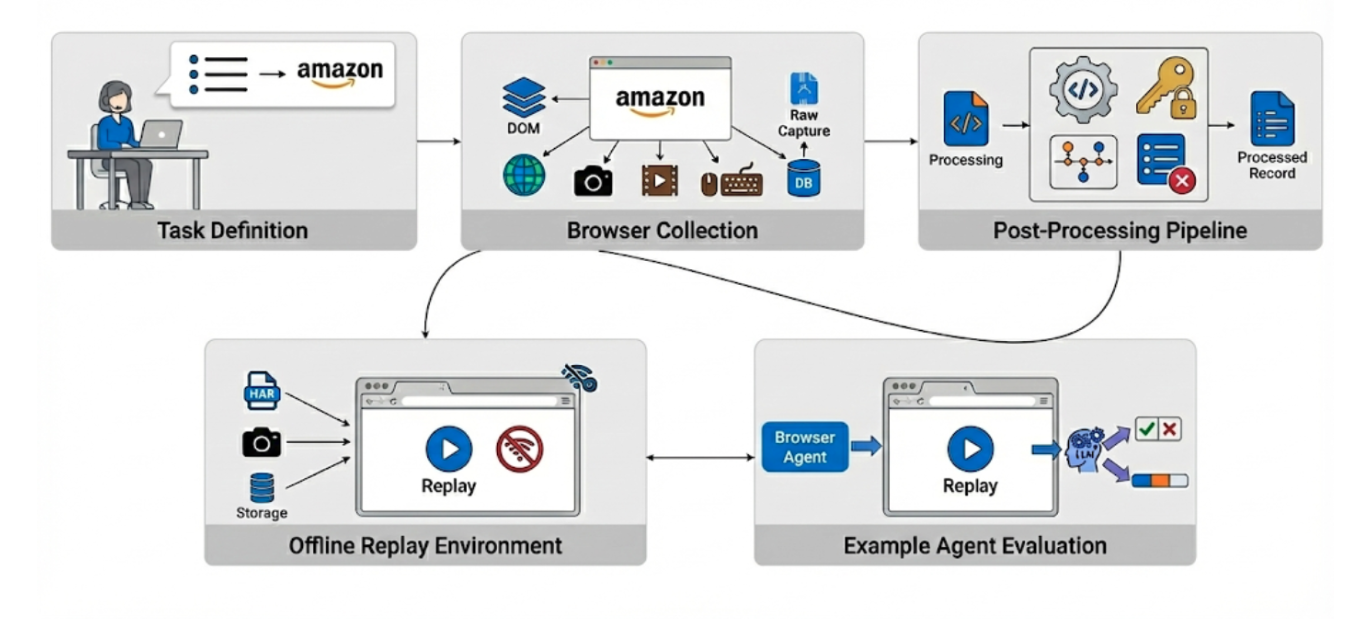
\includegraphics[width=\columnwidth]{01.png}
\caption{TRACE pipeline: collection, post-processing, offline replay, and agent evaluation.}
\label{fig:pipeline}
\end{figure}

\subsection{Collection Architecture}

TRACE's collection system is built on Playwright with a stealth-configured Chromium browser designed to avoid anti-automation detection while maintaining full recording fidelity.

\paragraph{Browser Configuration.} The collector launches Chromium with carefully selected arguments to evade bot detection:

\begin{lstlisting}
--disable-blink-features=AutomationControlled
--disable-features=VizDisplayCompositor
--no-sandbox
--disable-web-security
--enable-automation=false
\end{lstlisting}

The context is configured with realistic defaults: 1366$\times$768 viewport, \texttt{en-US} locale, \texttt{America/New\_York} timezone, and standard HTTP headers.

\paragraph{Event Recording.} The \texttt{Recorder} class captures events across multiple categories:

\begin{table}[h]
\caption{Event categories captured by TRACE.}
\small
\centering
\begin{tabular}{@{}lll@{}}
\toprule
\textbf{Category} & \textbf{Event Types} & \textbf{Trigger} \\
\midrule
State:Page & load, domcontentloaded & Page lifecycle \\
State:Browser & navigated, back & Navigation \\
Action:User & click, input, submit & User interactions \\
\bottomrule
\end{tabular}
\end{table}

For each triggering event, the recorder captures: (1) an accessibility snapshot (YAML-formatted tree of up to 400 interactive elements), (2) screenshots via Chrome DevTools Protocol, (3) full HAR network recording, and (4) browser state (cookies, localStorage, sessionStorage).

\begin{figure}[h]
\centering
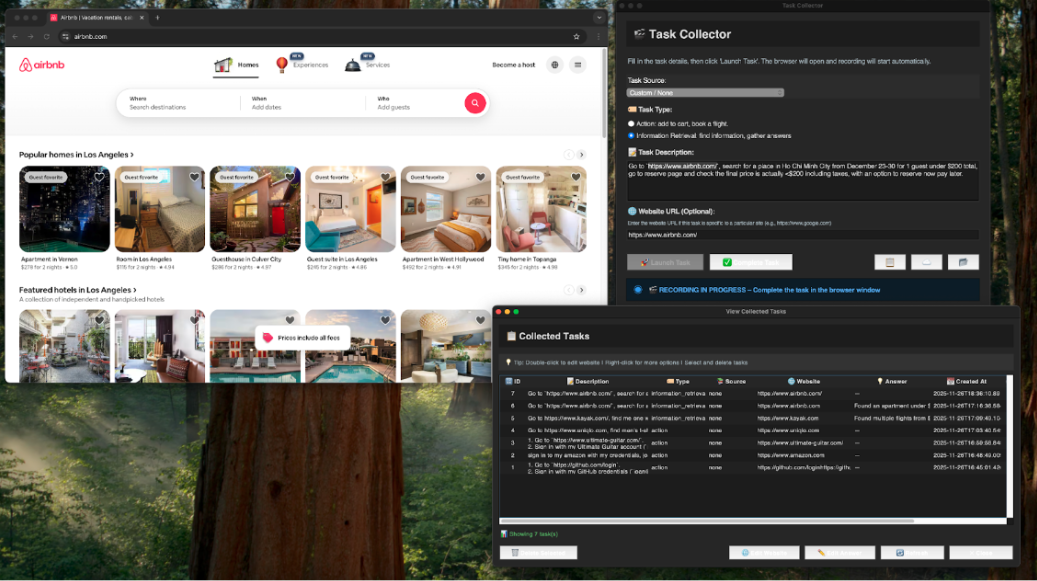
\includegraphics[width=\columnwidth]{03.png}
\caption{Collecting a task using the Tkinter desktop app.}
\label{fig:collection}
\end{figure}

\paragraph{Data Storage.} Each collection produces: SQLite database with task metadata, per-step DOM snapshots, screenshots, video recordings, and a capture bundle containing manifest, HAR file, storage state, and cached resources.

\subsection{Post-Processing Pipeline}

The post-processing pipeline transforms raw captures into clean artifacts through four stages:

\paragraph{Stage 1: Tool-Call Parsing.} Raw browser events are converted to a standardized DSL (\texttt{go\_to}, \texttt{click}, \texttt{type}, \texttt{scroll}) with element information and navigation consequences.

\paragraph{Stage 2: Credential Extraction.} An LLM-based extractor identifies credential-related interactions by analyzing tool calls and DOM context. Extracted credentials are stored separately, enabling credential substitution during sharing.

\paragraph{Stage 3: Checkpoint Selection.} An LLM analyzes the full trajectory to identify 2--3 semantically meaningful intermediate states suitable for partial-credit evaluation.

\paragraph{Stage 4: Ignore-List Construction.} Network traffic is analyzed to identify hosts and URL patterns that can be safely omitted (analytics, ad networks, non-essential third-party services). This stage discards approximately 50\% of captured HTTP requests.

\subsection{Replay Engine}

The replay module reconstructs captured sessions through multi-stage request matching:

\begin{figure}[h]
\centering
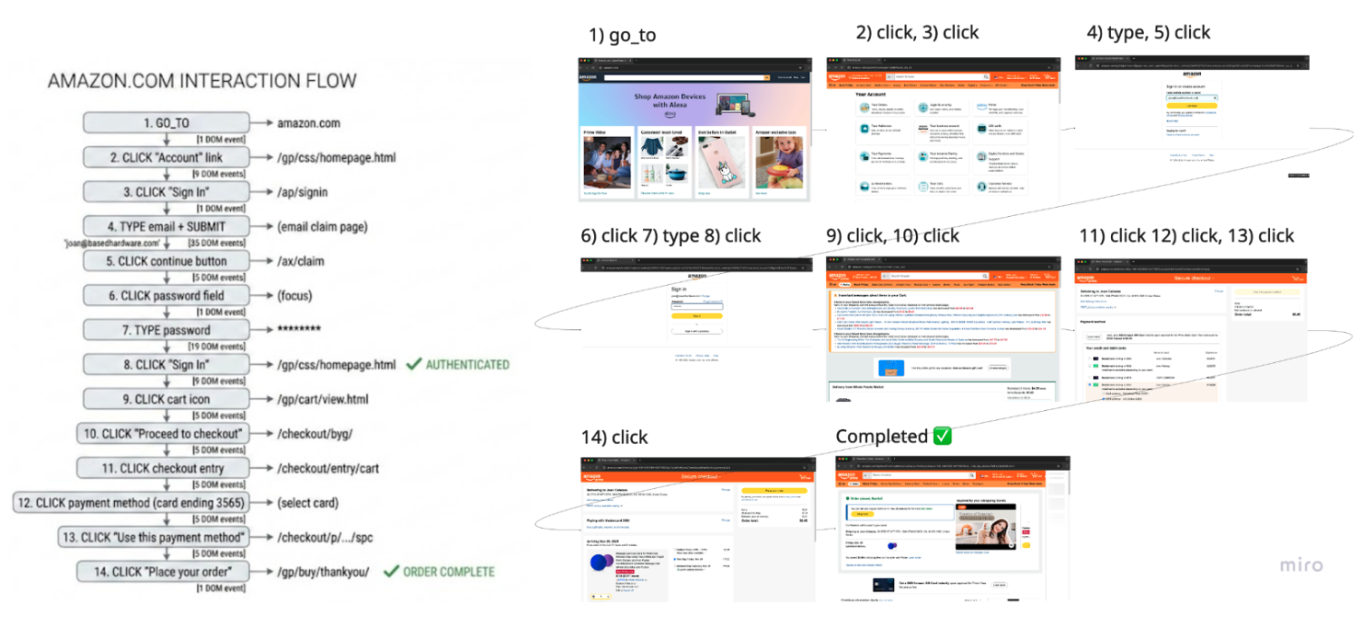
\includegraphics[width=\columnwidth]{05.png}
\caption{Offline replay and tool-call parsing for an Amazon task.}
\label{fig:replay}
\end{figure}

\paragraph{Request Routing.} When the browser issues a request during replay: (1) URLs matching ignore patterns are aborted; (2) exact matches on method and URL base are used directly; (3) character-frequency similarity scores handle dynamic query parameters; (4) LLM disambiguation resolves remaining ambiguities.

\paragraph{Response Fulfillment.} Once a HAR entry is selected, response headers are extracted, bodies decoded, and the request fulfilled via Playwright's route API.

\paragraph{Caching.} LLM match decisions are cached for determinism. The \texttt{--ignore-cache} flag forces fresh matching for debugging.

\subsection{Evaluation Harness}

TRACE includes a minimal evaluation runner: (1) load capture bundle and configure HAR replay routing; (2) initialize agent with task description; (3) compare agent trajectory against human checkpoints using semantic similarity; (4) assess binary success against expected outcome.

%%%%%%%%%%%%%%%%%%%%%%%%%%%%%%%%%%%%%%%%%%%%%%%%%%%%%%%%%%%%%%%%%%%%%%%%%%%%%%%%

\section{Captured Environment Statistics}
\label{app:statistics}

\begin{table*}[t]
\caption{Complete statistics for the six captured demonstration environments.}
\label{tab:stats}
\vskip 0.1in
\centering
\small
\begin{tabular}{@{}clccccccccc@{}}
\toprule
\textbf{Task} & \textbf{Website} & \textbf{Type} & \textbf{Clicks} & \textbf{Tools} & \textbf{Creds} & \textbf{HTTP} & \textbf{Cache} & \textbf{Shots} & \textbf{Time(s)} & \textbf{Size} \\
\midrule
1 & github.com & Action & 11 & 8 & Yes & 715 & 311 & 12 & 39.0 & 64 MB \\
2 & amazon.com & Action & 14 & 11 & Yes & 1,199 & 468 & 20 & 69.2 & 94 MB \\
3 & ultimate-guitar.com & Action & 19 & 15 & Yes & 2,752 & 534 & 20 & 54.9 & 117 MB \\
4 & uniqlo.com & Action & 11 & 10 & No & 1,315 & 783 & 12 & 46.1 & 128 MB \\
5 & kayak.com & Info & 14 & 11 & No & 816 & 452 & 32 & 110.7 & 154 MB \\
6 & airbnb.com & Info & 15 & 12 & No & 928 & 544 & 24 & 103.9 & 106 MB \\
\bottomrule
\end{tabular}
\end{table*}

\paragraph{Column definitions:}
\begin{itemize}
    \item \textbf{Clicks:} Number of click events recorded
    \item \textbf{Tools:} Number of high-level tool calls after post-processing
    \item \textbf{Creds:} Whether the task involved credential entry
    \item \textbf{HTTP:} Total HTTP request/response pairs (before filtering)
    \item \textbf{Cache:} Number of cached static resources
    \item \textbf{Shots:} Number of screenshots captured
    \item \textbf{Time(s):} Task execution duration in seconds
    \item \textbf{Size:} Total capture bundle size on disk
\end{itemize}

\paragraph{Aggregate totals:} Total HTTP requests: 7,725; Total cached resources: 3,092; Total screenshots: 120; Total storage: 663 MB.

\paragraph{Note on collection time:} The Time(s) column reflects successful execution duration. Actual collection effort averages $\sim$6:40 per task accounting for retries. The six-task dataset required about 40 minutes total.

\subsection{Task Descriptions}

\textbf{Task 1: GitHub (Authenticated).} Sign in, star a repository, search for and follow a user. Exercises authentication, navigation, and account actions.

\textbf{Task 2: Amazon (Authenticated).} Sign in, navigate to deals, find discounted item, add to cart, proceed toward checkout. Exercises e-commerce workflow including authentication, filtering, and cart management.

\textbf{Task 3: Ultimate Guitar (Authenticated).} Sign in, search for tabs, interact with playback controls. Exercises authentication on media-heavy site.

\textbf{Task 4: Uniqlo (Unauthenticated).} Browse catalog, apply filters, view product details, add to cart. Exercises e-commerce browsing without authentication.

\textbf{Task 5: Kayak (Information Retrieval).} Search flights with constraints, apply filters, compare results. Exercises travel search with complex filtering.

\textbf{Task 6: Airbnb (Information Retrieval).} Search accommodations with filters, browse listings with map interaction. Exercises map-based search with filtering.

%%%%%%%%%%%%%%%%%%%%%%%%%%%%%%%%%%%%%%%%%%%%%%%%%%%%%%%%%%%%%%%%%%%%%%%%%%%%%%%%

\section{Ethical and Safety Guidelines}
\label{app:ethics}

This appendix proposes guidelines for responsible capture and distribution of browser environments.

\subsection{Legal Considerations}

\paragraph{Copyright.} Captured environments contain copyrighted material. Fair use doctrines may permit research use, but this is untested for AI training. We recommend documenting fair use rationale and limiting distribution to research contexts. Notably, replica-based benchmarks face identical concerns: WebArena reproduces Reddit's interface; REAL simulates commercial sites.

\paragraph{Terms of service.} Most websites prohibit automated access in ToS, though enforceability varies (\emph{hiQ v. LinkedIn}). We recommend avoiding high-volume systematic capture and respecting robots.txt.

\paragraph{CFAA considerations.} Post-\emph{Van Buren} (2021), mere ToS violations are not CFAA crimes, but circumventing access controls may be. Capture only from accounts you own or have authorization to use.

\subsection{Privacy and Data Protection}

\begin{enumerate}
    \item \textbf{Informed consent.} Demonstrators should consent to capture and distribution.
    \item \textbf{PII detection and redaction.} Post-processing should detect and redact names, emails, addresses, financial data, and government identifiers.
    \item \textbf{Third-party minimization.} Avoid capturing pages with extensive third-party PII unless necessary.
    \item \textbf{Credential extraction.} TRACE separates authentication data from content; extend this to general PII.
\end{enumerate}

\subsection{Security Risks}

\paragraph{Credential exposure.} Captures may contain passwords, session cookies, API keys. Mitigations: mandatory credential extraction, secure storage, credential rotation after capture, preference for short-lived tokens.

\paragraph{Vulnerability disclosure.} Captures may reveal security flaws. Review captures before distribution; establish responsible disclosure procedures.

\subsection{Misuse Potential}

Capture-replay has dual-use risks. Environments could train agents for automated fraud, credential stuffing, or phishing.

\paragraph{Mitigations:} Access controls for sensitive domains; licensing that prohibits malicious applications; consider whether certain environment types should be captured at all; tiered access balances openness with responsibility.

\paragraph{Our view:} Proprietary concentration does not eliminate misuse risk; it prevents independent safety research. Transparent infrastructure enables collective norm development.

\subsection{Three-Tier Consent Framework}

\begin{table}[h]
\caption{Proposed consent framework for captured environments.}
\small
\centering
\begin{tabular}{@{}p{1.2cm}p{2cm}p{2cm}p{2cm}@{}}
\toprule
\textbf{Tier} & \textbf{Scope} & \textbf{Requirements} & \textbf{Distribution} \\
\midrule
1: Self & Own accounts & Consent, cred extraction & Public after processing \\
2: Auth & Others' demos & IRB, written consent, PII redaction & Research license \\
3: Sensitive & Healthcare, finance, govt & Domain compliance, legal review & Institutional agreements \\
\bottomrule
\end{tabular}
\end{table}

\subsection{Domain-Specific Notes}

\begin{itemize}
    \item \textbf{Healthcare:} Never capture real patient data; treat as Tier 3
    \item \textbf{Financial:} Stop before payment completion; never capture real card data
    \item \textbf{Government:} Jurisdiction-specific regulations apply
    \item \textbf{Enterprise SaaS:} Obtain written authorization from system owners
\end{itemize}

\subsection{Limitations}

These guidelines are not legal advice, cannot anticipate all risks, and depend on community adoption. Despite limitations, explicit guidelines are preferable to the implicit norms around replicas.

\end{document}
